%
Many decisions today are increasingly enabled by machine learning (ML) models.
Algorithmic decision-making (ADM) is becoming ubiquitous and its societal discontents clearer \parencite{Angwin2016MachineBias, DastinAmazonSexist, Heikkila2022_DutchScnadal}. 
There is a shared urgency by regulators and researchers alike to develop frameworks that asses these ML models for potential discrimination based on protected attributes such as gender, race, and religion \parencite{Kleinberg2019DiscAgeOfAlgo, DBLP:conf/aaai/Ruggieri0PST23, DBLP:journals/ethicsit/AlvarezCEFFFGMPLRSSZR24}. 
Discrimination is often conceived as a causal claim on the effect of the protected attribute over an individual decision outcome \parencite{Heckman1998_DetectingDiscrimination}. It is, in particular, a conception based on counterfactual reasoning---what would have been the ML model outcome if the individual, or \textit{complainant}, were of a different protected status?---where we ``manipulate'' the protected attribute of the individual. \textcite{Kohler2018CausalEddie} calls such conceptualization of discrimination the \textit{counterfactual causal model of discrimination} (CMD). 

Most frameworks for proving discrimination are based on the CMD. 
Central to these frameworks is defining similar instances to the complainant; arranging them based on their protected status into control and test groups; and comparing the decision outcomes of these two groups to detect the effects of the protected attribute. 
Among the available frameworks \parencite{Romei2014MultiSurveyDiscrimination,DBLP:journals/jlap/MakhloufZP24, DBLP:journals/fdata/CareyW22}, however, there is a need for one that is both \textit{actionable} and \textit{meaningful}. 
% We consider a framework to be 
A framework is actionable if it rules out random circumstances from the discrimination claim as required by courts (e.g.,~\textcite{Foster2004, EU2018_NonDiscriminationLaw, Nachbar2020algorithmic}) and meaningful if it accounts for known links between the protected attribute and all other attributes 
% when manipulating the former 
as demanded by social scientists (e.g.,~\textcite{Bonilla1997_RethinkingRace, Sen2016_RaceABundle, Kasirzadeh2021UseMisuse}).
%
In practice, we view actionability as an inferential concern to be handled by comparing multiple control-test instances around a complainant, while meaningfulness as an ontological concern to be handled by requiring domain-knowledge on the protected attribute and its effect on the other attributes of the complainant.

In this work, we present \textit{counterfactual situation testing} (CST), a causal data mining framework for detecting individual cases of discrimination in a dataset of classifier decisions.
% The dataset can be the one used to train a ML model, or it can also be the dataset of actual decisions by a ML model.
The dataset can be the one used to train a ML model or the one of actual decisions by a ML model. 
In the former case we want to prevent learning discriminatory patterns, while in the latter case we want to detect discriminatory decisions.
%
The goal of CST is to be both an actionable and meaningful framework.
It combines (structural)\footnote{Not to be confused with counterfactual explanations \parencite{Wachter2017Counterfactual}. \textcite{Karimi2021_AlgoRecourse}, e.g.,~use ``structural'' to differentiate counterfactuals from counterfactual explanations.} 
counterfactuals \parencite{PearlCausality2009} with situation testing \parencite{Thanh_KnnSituationTesting2011}.
%
\textit{Counterfactuals} answer to counterfactual queries, such as the one motivating the CMD, and are generated via structural causal models. 
Under the right causal knowledge, counterfactuals reflect at the individual level how changing the protected attribute affects other seemingly neutral attributes of a complainant.
%
\textit{Situation testing} is a data mining method, based on the homonymous legal tool \parencite{Bendick2007SituationTesting, Rorive2009_ProvingDiscrimination}. 
For each complainant, given a search algorithm and distance function for measuring similarity, situation testing finds and compares a control and test group of similar protected and non-protected instances in the dataset, where a difference between the decision outcomes of the groups implies potential discrimination.
Hence, \textit{CST follows the situation testing pipeline with the important exception that it constructs the test group around the complainant's counterfactual instead of the complainant.}
To illustrate CST and how it compares to standard situation testing, let us use Example~\ref{ex:IllustrativeExample} below.

%
\begin{example}(An illustrative example)
\label{ex:IllustrativeExample}
    Let us consider the scenario in Figure~\ref{fig:KarimiV2} in which a bank uses the classifier $b$ to accept or reject ($\hat{Y}$) individual loan applications based on annual salary ($X_1$) and account balance ($X_2$), such that $b(X_1, X_2) = \hat{Y}$. 
    Suppose a female applicant ($A=1$) with $x_1= 35000$ and $x_2=7048$ is rejected and files for gender discrimination. 
    According to Figure~\ref{fig:KarimiV2}, the bank uses non-sensitive information to calculate $\hat{Y}$, but there is also a ``known'' link between $A$ and $\{X_1, X_2\}$ that questions the neutrality of the information. 
    %
    \textit{Under situation testing}, we find a number of females and males with similar characteristics in terms of $X_1$ and $X_2$ to the complainant and compare them.
    Comparing multiple instances allows to check whether the complainant's claim is representative of an unfavorable pattern toward female applicants by the model (i.e.,~actionability). 
    % On the other hand, 
    However, knowing what we know about $A$ and its influence on $X_1$ and $X_2$, would it be fair to compare these similar females and males? 
    As argued by works like \textcite{Kohler2018CausalEddie}, the answer is no as this \textit{idealized comparison} 
    % underpinning situation testing 
    takes for granted the effect of $A$ on $X_1$ and $X_2$ by allowing the former to change while expecting the latter two to remain the same despite the known links.
    %
    \textit{Under counterfactual situation testing}, instead, we generate the complainant's counterfactual using the auxiliary causal knowledge, creating a male applicant with a higher $x_1=50796$ and $x_2=13852$, and use him 
    % rather than the complainant 
    to find similar male instances for constructing the test group.
    The resulting control and test groups have similar $X_1$ and $X_2$ within them but different $X_1$ and $X_2$ between them. 
    This disparate comparison embodies \textit{fairness given the difference}, explicitly acknowledging the lack of neutrality when looking at $X_1$ and $X_2$ based on $A$ (i.e.,~meaningfulness).
    We come back to this example in Section~\ref{sec:Experiments}.
\end{example}
%

%
\begin{figure}[t]
\begin{minipage}{.45\linewidth}
\begin{figure}[H]
\centering
    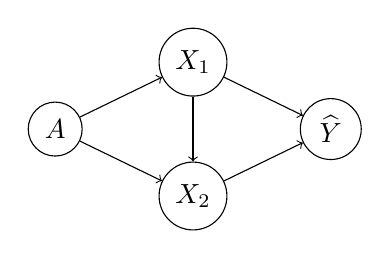
\begin{tikzpicture}
        \node (A)  at (-1.75, 0) [circle, draw]{$A$};
        \node (X1) at (0, 0.85) [circle, draw]{$X_1$};
        \node (X2) at (0,-0.85) [circle,draw]{$X_2$};
        \node (Y)  at (1.75, 0) [circle, draw]{$\widehat{Y}$};
        \draw[->] (A) to (X1) {};
        \draw[->] (A) to (X2) {};
        \draw[->] (X1) to (Y) {};
        \draw[->] (X1) to (X2) {};
        \draw[->] (X2) to (Y) {};
    \end{tikzpicture}
\end{figure}
\end{minipage}
\begin{minipage}{.45\linewidth}
\begin{align*}
\mathcal{M} \, & 
\begin{cases}
    A & \leftarrow U_{A} \\
    X_1 & \leftarrow f_1(A)  + U_1 \\
    X_2 & \leftarrow f_2(X_1, A) + U_2
\end{cases}
\end{align*}
\begin{align*}
    \widehat{Y} & = b(X_1, X_2) 
    % \\
    % & = \mathbbm{1}\{ X_1 + 5 \cdot X_2 > 225000\}
\end{align*}
\end{minipage}
\caption{The auxiliary causal knowledge for Example~\ref{ex:IllustrativeExample} (and Section~\ref{sec:Experiments.IllustrativeExample}). Let $A$ denote gender, $X_1$ annual salary, $X_2$ account balance, and $\widehat{Y}$ the loan decision by $b()$. It consists of a causal graph (left) and a set of structural equations (right), both introduced in Section~\ref{sec:CausalKnowledge}.}
\label{fig:KarimiV2}
\end{figure}
% 

We evaluate the CST framework on synthetic and real ADM datasets.
We use a k-nearest neighbor implementation of the framework, k-NN CST, to compare it to its situation testing counterpart, k-NN ST, by \textcite{Thanh_KnnSituationTesting2011}.
The $k$ denotes the number of instances for each control and test groups, determining the size of the many-to-many comparison of each complainant in the dataset.
Our experiments show that CST detects a higher number of individual discrimination cases across different $k$ sizes. 
The results illustrate the impact of moving from the idealized comparison of the k-NN ST to the fairness given the difference comparison of the k-NN CST.
This last point is important as legal scholars continue to call for an alternative to the idealized comparison \parencite{Kohler2018CausalEddie}.
Importantly, we consider single and multidimensional discrimination, meaning, respectively, claims based on one and many protected attributes.
While single discrimination testing is commonly studied, multidimensional discrimination testing is largely unexplored and often portrayed as a straightforward extension to single discrimination testing \parencite{Xenidis2020_TunningEULaw}.

Multidimensional discrimination covers two forms: multiple and intersectional. 
In multiple discrimination the complainant must be discriminated for each of the protected attributes, while in intersectional discrimination the complainant must be discriminated at the intersection of the protected attributes.
To illustrate this distinction, suppose the complainant in Example~\ref{ex:IllustrativeExample} is also non-white and makes a claim based on gender and race. 
Multiple discrimination occurs if the complainant is discriminated, separately, as a female and as a non-white individual.
Intersectional discrimination occurs if the complainant is discriminated, simultaneously, as a female-non-white individual.
Each form of multidimensional discrimination, in turn, poses different problem formulations for discrimination testing \parencite{DBLP:conf/fat/0001HN23, WangRR22}.
Beyond the distinct problem formulations, an open issue with these two forms of discrimination is that only multiple discrimination is recognized by non-discrimination law. 
Legal scholars have raised concerns on this lack of recognition for intersectional discrimination, arguing that multiple discrimination fails to account for it \parencite{Xenidis2020_TunningEULaw}.
We test for multiple and intersectional discrimination using CST, finding that the former does not capture the latter.
This work is the first to evaluate and provide evidence for this legal concern.

Additionally, CST provides an actionable extension to \textit{counterfactual fairness} by \textcite{Kusner2017CF}, which remains the leading causal fair ML definition \parencite{DBLP:journals/jlap/MakhloufZP24}.
A ML model is counterfactually fair when the complainant's and its counterfactual's decision outcomes are the same. 
These are the same instances used by CST to construct, respectively, the control and test groups, which allows to equip this popular fairness definition with measures for uncertainty due to the many-to-many comparison. 
CST links counterfactual fairness claims with statistical significance, and
positions it for discrimination testing as uncertainty measures are often required by courts \parencite{EU2018_NonDiscriminationLaw}.
By looking at the control and test groups rather than the literal comparison of the factual versus counterfactual instances, CST evaluates whether the counterfactual fairness claim itself is representative of similar instances.
Our results show that individual discrimination can occur even when the ML model is counterfactually fair, capturing the scenario where a model discriminates when evaluating borderline instances.

In summary,
with CST we present a meaningful and actionable framework for detecting individual discrimination.
Our main contributions are threefold.
%
First, we offer the first explicit operationalization of \textit{fairness given the difference} for discrimination testing and, in doing so, define a new view on similarity that is more flexible than the standard idealized comparison.
%
Second, we explore single and multidimensional discrimination testing, studying the latter's tension between multiple and intersectional discrimination.
%
Third, we equip counterfactual fairness with confidence intervals, introducing an actionable extension to the popular causal fairness definition.

The rest of the paper is organized as follows.
We present the related work in Section~\ref{sec:RelatedWork} and the role of auxiliary causal knowledge within CST for discrimination testing in Section~\ref{sec:CausalKnowledge}.
We introduce the CST framework in Section~\ref{sec:CST}, including its k-NN implementation.
We showcase CST using two classification scenarios in Section~\ref{sec:Experiments}.
We discuss the main limitations of this work in Section~\ref{sec:Discussion}.
We conclude in Section~\ref{sec:Conclusion}.

%
% EOS
%
